\documentclass[a4paper,12pt]{article}

\usepackage[utf8]{inputenc}
\usepackage[T1]{fontenc}
\usepackage[english]{babel}
\usepackage{geometry}
\usepackage{graphicx}

\geometry{margin=1in}

\title{Quiz Game Description}
\date{\today}

\begin{document}

\maketitle

\section{Introduction}
\subsection{How to compile project}
Ensure you have the following installed:
\begin{itemize}
    \item g++
    \item cmake
\end{itemize}

To compile there is needed cmake installed. Create \texttt{build/} directory\
in root, enter it and run \textbf{cmake ..} because CMakeLists.txt is in root.\
After running it in \texttt{build/compiled/} directory is executable file to\
run application.

\section{Game Description}
base idea:
The quiz game will be about testing the user's knowledge in various categories.\
The game will present single-choice questions. Questions will be presented one\
at a time.

\section{Implementation}
There will bew used MVC pattern.\
Header files will be used to separate classes and will be placed in the\
\texttt{include} folder with the same name as the class and in the folder with same name.\
Different categories of questions will be in different files.
\subsection{Model}
There will be all logic of the game. This will include:
\begin{itemize}
    \item Question class - this will be a base class for all questions
    \item Game class - this will be the main class of the game
    \item Player class - this will be a class for player
\end{itemize}
The question class will be a base class for all questions. In "Ideas for Future Development"\
there are some ideas connected with different types of questions - MVC will make it easier to\
add after implementing the base game.
\subsection{View}
Currently the view can be implemented in console.\
In future it can be in GUI. Splitting to different modules\
makes it easy to rebuild view without changing other components.\
This part will include classes:
\begin{itemize}
    \item Main menu class - class to display main menu
    \item Answering question view class - to display question and give posiibility to answer
    \item ViewManager - to manage what should be displayed
\end{itemize}
\subsection{Controller}
The controller will be responsible for communication between\
the model and the view. It will also handle the user input and\
update the model accordingly.\newline \newline

\begin{figure}[h]
    \centering
    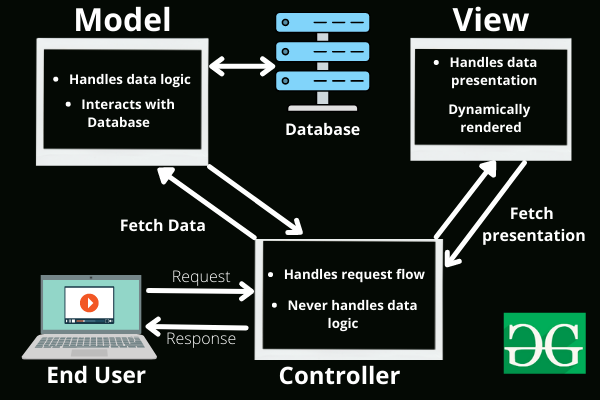
\includegraphics[width=0.5\textwidth]{images/Model1.png}
    \caption{The image represents the way like MVC should work.}
    \label{fig:class_diagram}
\end{figure}



\section{Technologies Used}
\begin{itemize}
    \item C++ - with STL libraries
    \item cmake - for building the project
    \item g++ - for compiling the project
    \item git - for version control
\end{itemize}

\section{Ideas for Future Development}
\begin{itemize}
    \item Add more question categories. - obviously, currently there are none
    \item Implement a scoring system. - maybe
    \item Create a user-friendly interface. - now is only needed simple or console
    \item Add a timer for each question. - maybe
    \item few categories of questions - knowledge or knowledge about another person
    \item Add multiplayer functionality. - category like in cozy app and category where like opponents
    \item Adding own questions - I think needed in the future
\end{itemize}
\end{document}